\documentclass[journal]{IEEEtran}

% correct bad hyphenation here
\hyphenation{op-tical net-works semi-conduc-tor}
\usepackage{graphicx}

\begin{document}

\title{Sensor Descriptive Movements for Localization}

\author{Zheng~Lu,
        Zhiyang~Zhang,
        and~Michael~Craze
\thanks{Z. Lu, Z. Zhang and M. Craze is with the Department
of Electrical Engineering and Computer Science, University of Tennessee, Knoxville,
TN, 37996 USA }} 

% The paper headers
\markboth{Final Project Report for Class ECE555, November~2012}%
{Shell \MakeLowercase{\textit{et al.}}: Intros to SDM}

\IEEEspecialpapernotice{(Invited Paper)}

\maketitle

\begin{abstract}
Currently smartphone apps are using GPS as their major source to acquire user's location. 
Due to the limitation of GPS in terms of energy efficiency and latency to fix a location, such apps will drain the battery in one or two hours and can hardly get responsive localization results. 
With the motivation of finding new ways to take advantage of sensors to improve our daily life, we propose to use sensors on modern smartphones to assist in keeping track of the movements of users to get better performance in localization applications. 
It is expected that by using sensors we can greatly reduce the usage of energy consuming GPS transceivers and can realize some location related applications with tight time constraints. 
We have then illustrated two possible applications which can take advantage of sensor data to describe user movements.
We focus on the path recording application in this paper.
We designed a sensor based path recording system that use the GPS to acquire the initial location and then use accelerometer and magnetometer readings to describe user movements.
With the aid of sensor readings, we can track and record user's location in real-time with very high energy efficiency.
We implement our SDM path recording system using python and deploy it in several modern Android smartphones and run a set of tests.
The result of our tests show that sensor aided localization can achieve certain level of accuracy with very few energy consumption.
\end{abstract}

\begin{IEEEkeywords}
Sensors, Movement monitoring, Tracking, Smartphones
\end{IEEEkeywords}

\section{Introduction}
\IEEEPARstart {D}{ue} to the fast development of sensor technologies and the world wide spread of smartphones, more and more sensors have been integrated into our smartphones nowadays. 
These sensors enable us to realize many brand new applications which can greatly make our daily life more fruitful. 
Our location information is crucial for some applications these days. 
Apps may provide more specialized information based on your location, such as route to specific places or path recordings of a trip.
In this paper, we are going to propose a novel approach to provide location information.

\subsection{Why not use the GPS?}
GPS and its variants take advantage of GPS satellites to provide high precision localization information \cite{GPS}. 
A GPS receiver which can receive broadcast signals from GPS satellites is usually very cheap nowadays. 
Thus it is widely integrated into smartphones and used as major approach to get user's location. 

But there are several drawbacks of GPS.
The first is that since it is a communication based approach, it will consume a lot of energy during localization. 
Since most embedded systems have very limited energy, this disadvantage makes it less practical in current embedded systems.
The second is that usually the startup performance is not very promising (as long as 12 minutes for regular GPS and dozens of seconds for A-GPS) \cite{A-GPS}, which means once you lose GPS signal, you will need quite a long time to get your location again. 
Not only the startup time of GPS is very high, the GPS signal receiver also suffers from hundred milliseconds level of latency \cite{GPS Latency}.
This disadvantage makes it less possible to use GPS in some tightly time-constrained applications. 

\subsection{How about the sensors?}
To reduce those disadvantages brought by GPS, we propose using sensors to describe human movements to help in acquiring location information. 
Currently, most smartphones are equipped with sensors such as accelerometers, magnetometers and gyroscopes, which are capable of describing movement. 
By periodically monitoring these sensors and cooperatively interpreting their readings, we can describe our movements with an acceptable accuracy. 
Once we get the movement description of users, we can calculate their current location together with their initial location which should be acquired though the GPS or even manually set. 
Through this approach, we can minimize the usage of the GPS to save energy or even implement some applications which have restricted time requirements that GPS cannot meet. 
There are already some mechanisms in the literature have used sensors in aiding locations, but the GPS is still turned on most of the time in their approach \cite{Sensor Aug}, \cite{Track for Mobile}.

The rest of the paper is organized as follows.
We will discuss two possible applications in Section II.
We study the measurements of energy consumption of the GPS and sensors, as well as sensor readings to analyze advantages of sensor based localization in Section III.
Section IV provides the system overview of the path recording application.
The design details of SDM path recording system are discussed in section V.
To verify our system, we implemented several experiments in section VI.
Finally, we conclude our results in section VII.

\section{Possible Applications}
We have proposed 2 specific sample applications here.

\begin{figure}
	\centering
	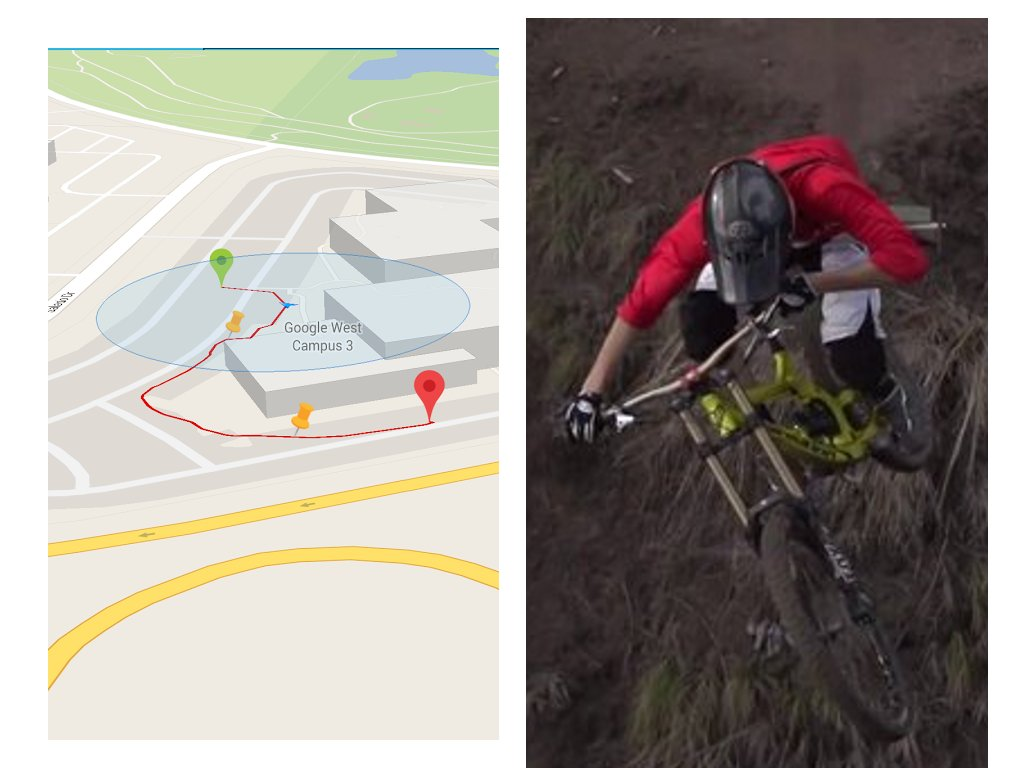
\includegraphics[width=3.5in]{figures/pic}
	\caption{(a) Path Recording Applications	(b) Personal Aerial Photography}
\end{figure}

\subsection{Personal aerial videotaping}
We emphasize on low latency to meet the restricted time constraints of applications. These applications can hardly be implemented by only using the GPS, please refer to Fig.1 (b) .

\subsection{Path recording}
We emphasize on energy efficiency compared to regular GPS based path recording applications such as Google's "My Tracks", please refer to Fig.1 (a) . 
The key idea in this application is that we will attempt to use sensor readings to decide the best time to turn on the GPS, while the GPS is off most of the time.
Our goal is to reduce the turning on time of the GPS as much as possible, so that more energy is saved. 

We will focus on this application in our following work. 

\section{The Measurements}
To verify the feasibility and effectiveness of our approach, we will study the energy consumption of the GPS and sensors, as well as data readings from sensors.
For the specific application of path recording, we will also discuss some possible auxiliary means to increase our accuracy without sacrificing energy efficiency.

\begin{figure}
	\centering
	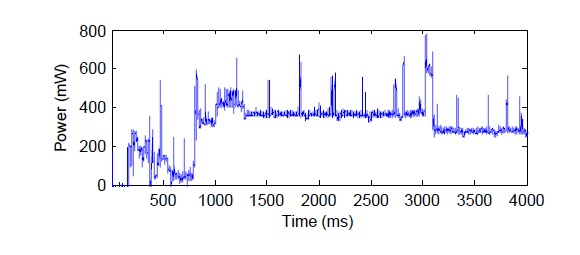
\includegraphics[width=3.5in]{figures/dpower}
	\caption{Detailed GPS power \cite{GPS Measurements} }
	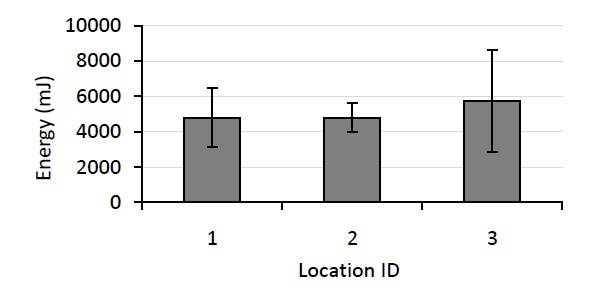
\includegraphics[width=3.5in]{figures/csenergy}
	\caption{GPS cold start energy consumption of different locations \cite{GPS Measurements} }
\end{figure}

\subsection{Energy consumption}
Before we try to reduce energy consumption by replacing the GPS with sensors as long as possible, we need to study the potential benefit of this method. 
This section studies the energy consumption of the GPS and sensors on smartphones to draw the potential energy saving of this approach. 

\subsubsection{Energy consumption of GPS} 
Reference \cite{GPS Measurements} gives a detailed measurement of energy consumption of the GPS on Android smartphones. 
The power draw of the GPS on Android systems has been measured at around 230mW compared to 324mW on Nokia N95. 
Please refer to Fig.2 for detailed energy consumption of the GPS. 
Also, the energy consumption of the GPS systems vary when measured from different locations.
Fig.3 shows the energy measurements of a cold start of GPS in different locations.
We can draw from Fig.3 that by using A-GPS, the cold start up time is around 25 seconds.
Note that the energy consumption will drop to one fourth when using a warm start, that is, the system has previous almanac or ephemeris data. 
Also, the warm start up time will be only around 6 seconds. 

\subsubsection{Energy consumption of sensors} 
While GPS cost large amount of energy, on the contrary, the sensors in smartphones require far less energy. 
Using iPhone 5s's accelerometer chip STMicroelectronics LIS331DLH as an example \cite{Acc Measurements}. 
Under 2.5v supply voltage, the current consumption under normal mode is only 250uA and under low-power mode, this value is decreasing surprisingly to only 10uA. 
This means that the power consumption of this accelerometer is less than 1mW, which is negligible compared to power consumption of the GPS. 

\subsubsection{Energy consumption of our approach} 
The sensor is absolutely more attractive with regards to energy consumption according to the energy measurements above. 
In our implementation, we are considering using GPS signal discontinuously and using sensor readings to aid in locating when the GPS is off. 
It is beneficial if we can always use a warm start up after the first start. The minimal interval for us to turn on the GPS should be larger than the warm start up time, that is, 6 seconds on average.
Also, according to the detailed energy consumption in Fig.2, GPS does not consume much more energy at start up than in it's stable state. 
So, we can turn it off arbitrarily without facing any punishment in terms of energy consumption, but we may face a latency averaged at 6s when we try to get a location from GPS.
To conclude, the energy consumption of our method for locating is dominant by the power on time of GPS.

\subsection{Characteristics of sensor readings}
In this section, we design several simple tests to study whether the characteristics of sensor readings are suitable for our tracking purpose.
During tests, we wrote a script running on an Android smartphone to periodically record accelerometer and magnetometer readings. 

\subsubsection{Characteristics of sensor readings while static}
\begin{figure}
	\centering
	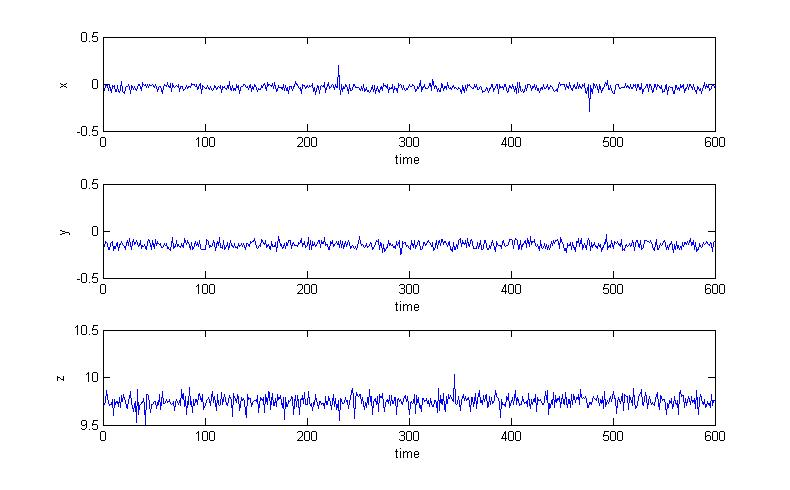
\includegraphics[width=3.5in]{figures/acc-stay}
	\caption{Accelerometer readings of xyz coordinates while static}
	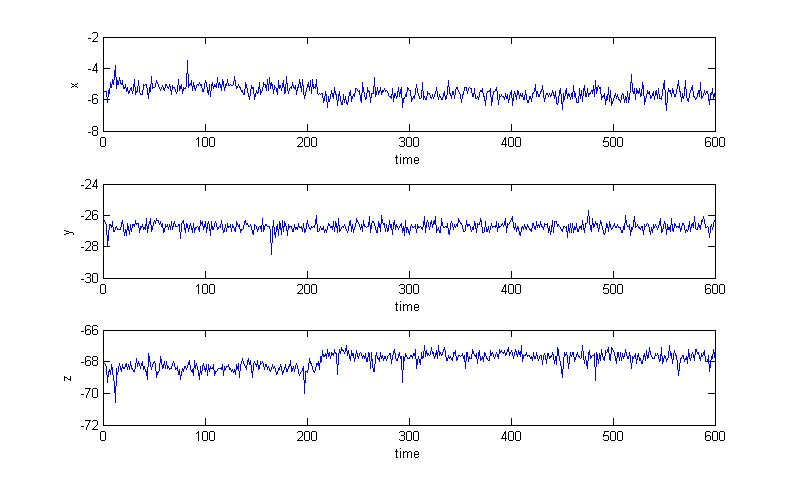
\includegraphics[width=3.5in]{figures/mag-stay}
	\caption{Magnetometer readings of xyz coordinates while static}
\end{figure}

First we examine the sensor readings while it has been put on the desk.
This will help us to see the errors introduced by the sensors itself.
From Fig.4 and Fig.5 we can see that both accelerometer readings and magnetometer readings is pretty stable, there is no significant errors there.

\subsubsection{Characteristic of sensor readings while walking}
\begin{figure}
	\centering
	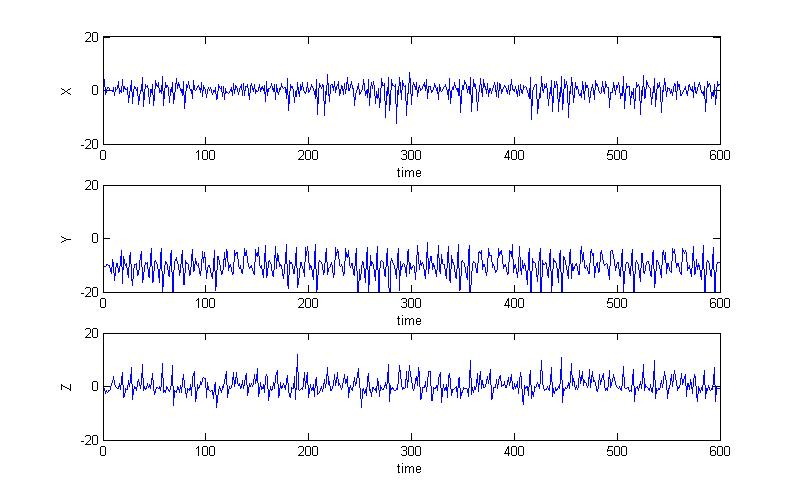
\includegraphics[width=3.5in]{figures/AccTest}
	\caption{Accelerometer readings of xyz coordinates during the walk}
	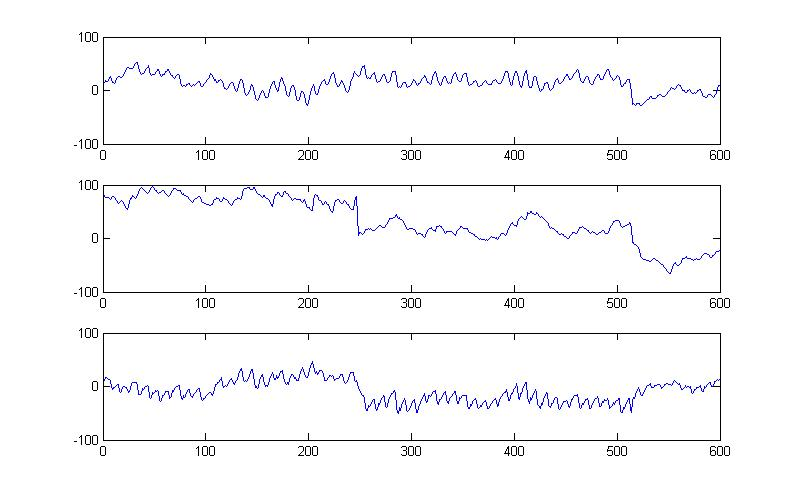
\includegraphics[width=3.5in]{figures/MagTest}
	\caption{Magnetometer readings of xyz coordinates during the walk}
\end{figure}

We then test the sensor readings in a walking scenario.
We put the smartphone into the left pocket of pants and walking in the Min Kao fourth floor.
We took two turns during the test.

The result from Fig.6 seems chaotic at the first look, but when we look into it, we may draw some really useful information:

\begin{itemize}
	\item orientation of smartphone: 

		we can estimate the orientation of the cell phone, since the y-axis is always around minus 10, which means that is the gravity.
	\item orientation of moving: 

		since in most of the time, the sensor readings of the y-axis and z-axis are near symmetric of their mean values, we can learn that the person carrying the smartphone is moving along the x-axis.
	\item direction of moving: 

		since the value is larger towards the negative direction of x-axis, which means that we are approximately moving towards the minus x-axis direction.
\end{itemize}

The readings of the magnetometer from Fig.7 has more obvious trends compared to the readings of the accelerometer. 
We can draw the following information from its readings (note that the accelerometer and magnetometer are not necessarily share the same coordinates system):

\begin{itemize}
	\item orientation of smartphone: 

		we can estimate the orientation of the smartphone, this can help us using accelerometer and magnetometer cooperatively to more precisely determine the orientation of smartphone.
	\item orientation of turns: 

		more interesting result from the magnetometer readings is that we can tell the direction of our turns with these readings. 
		We are turning two times in this test scenario, you can find obvious clues of this two turns especially from y-axis.
\end{itemize}

From above results and analysis, we can conclude from this experiment that we can draw sufficient information from sensor readings to describe our movements and assist in localization when the GPS is off. 

Although, we can also see that since the sensor readings are suffering from volatiles because of the nature of our moving pattern, we can not calculate accurate movements and locations through these sensor readings.
So the GPS is still necessary for the precise path recording of our approach.

\subsubsection{Characteristic of sensor readings while biking}
\begin{figure}
	\centering
	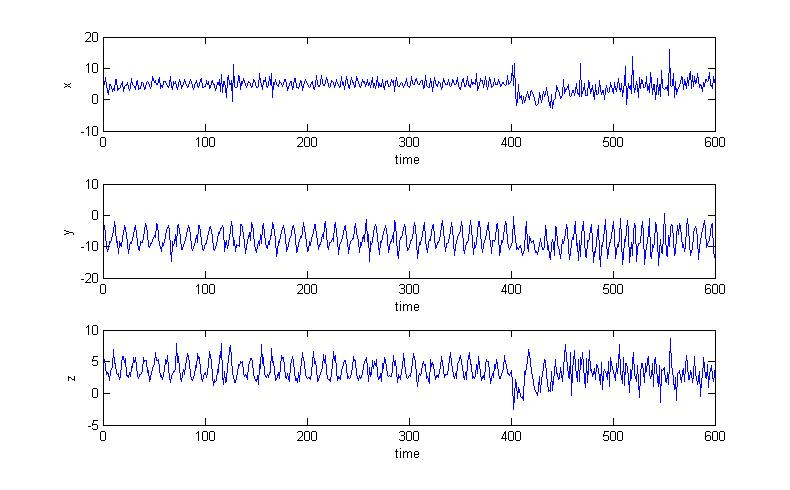
\includegraphics[width=3.5in]{figures/acc-biking}
	\caption{Accelerometer readings of xyz coordinates during the ride}
	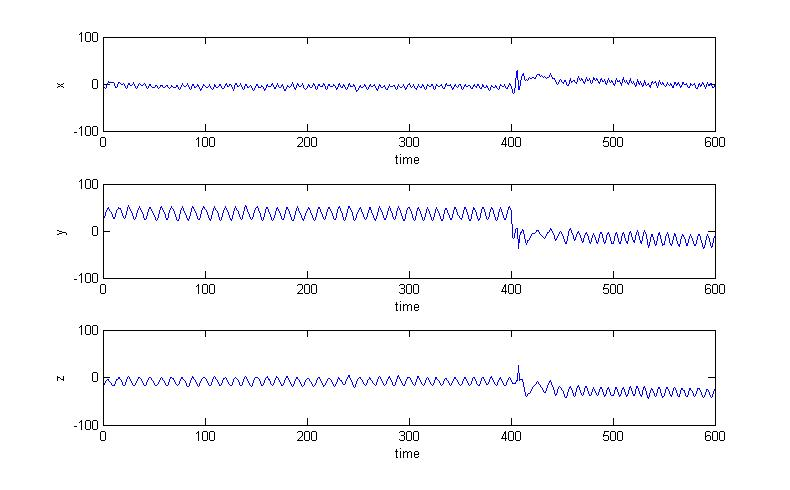
\includegraphics[width=3.5in]{figures/mag-biking}
	\caption{Magnetometer readings of xyz coordinates during the ride}
\end{figure}

We ride on a flat road first, then after a turn, we ride on a little ascending road.
The results are shown in Fig.8 and Fig.9.
The accelerometer readings are very good at the first 400 samples, which we are riding on a flat road and pedal gently.
The accelerometer readings are kind of volatile at the last 200 samples, which we are riding on an ascending road and pedal hardly.
The magnetometer readings are very promising during this test, Which we believe because the magnetic field is quite constant outside and pedalling will introduce far less shocks than walking.

\subsection{An auxiliary method to improve accuracy}
The google map on Android systems provides a function called geocoding, which we can use the coordinates we have to get the information of the road. 
So when we use the path recording application in a city scenario, we can define our location result on the road.
This method can reduce the effect of volatile sensor readings to the accuracy of the localization without incurring large energy consumption compared to acquiring location from the GPS.

\section{System Overview}
Our goal is to deliver a low energy consumption, real-time accurate path recording system.
We will split our system into four parts according to their functionality, namely central controller, sensor data interpreter, map integrator, GPS coordinator.

\subsection{Non-functional requirements}
We will talk about the most important non-functional requirements in this section:

\begin{itemize}
	\item low power: 

		The major concern of our system is its power consumption. That is the main reason we sacrifice simplicity of only using the GPS.
	\item real-time: 

		Since sensors do not suffer from high energy localization refresh overhead and long latency due to poor connection. 
		So we are expecting that our approach outperforms those only using the GPS in terms of real-time in some scenarios such as urban areas, forests.
	\item accuracy: 

		The most significant drawback of sensor approach is its poor accuracy. 
		Although we can always increase the frequency of using the GPS to achieve a better accuracy, this will reduce the benefit of our approach.
		We hope we can overcome low accuracy issue through better sensor readings interpreting algorithm design.
\end{itemize}

\subsection{The SDM Path Recording System Architecture}
\begin{figure}
	\centering
	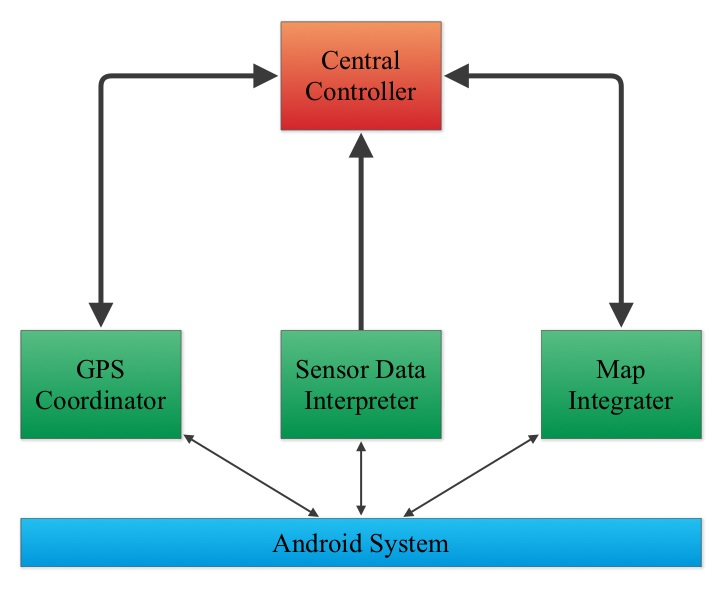
\includegraphics[width=3.5in]{figures/sysArc}
	\caption{System architecture}
\end{figure}

Fig. 10 shows the system architecture of our SDM path recording system.
We will talk about the functionality of each component of our system in this section.

\subsubsection{Central controller}
The central controller is where we keep the main logic of our system. 
Other components are all connected to this component. 
The central controller will monitor the possible localization errors in our algorithm by combining movement descriptions from  sensor data interpreter and map auxiliary information from the map integrator.
It will also determine the frequency of using the GPS.
This component will also provide the user interface.

\subsubsection{Sensor data interpreter}
This is the major part of our system. 
It contains the algorithm of interpreting the sensor readings into movement descriptions. 
It will provide this information to the central controller.

\subsubsection{Map integrator}
This component has two functions. 
The first is to recording coordinates provided by central controller on the map.
The second is to provide the map auxiliary information to the central controller to help determine the coordinates.

\subsubsection{GPS coordinator}
This component coordinates with the GPS to manage the usage of the GPS.
It will provide coordinates acquired from the GPS to the central controller upon request.

\subsection{The SDM Path Recording System Work Flow}
\begin{figure}
	\centering
	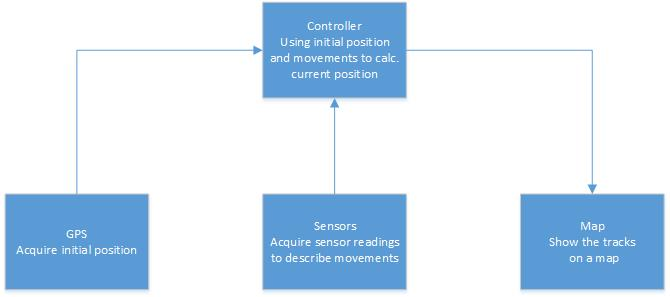
\includegraphics[width=3.5in]{figures/workflow}
	\caption{System work flow}
\end{figure}

Fig.11 shows the work flow of our SDM path recording system.
The detailed explanations are as follows:

The central controller will call the GPS coordinator to get the coordinates of initial location.
After that, it will use the movement description data from sensor interpreters to update the coordinates.
When the movement description data yields a significant direction change, the central controller will call the GPS to calibrate current coordinates.
For an online approach, the recorded coordinates will be sent to the map integrator to show them on the map as dots and use straight lines to connect them.
For an offline approach, the recorded coordinates will be stored in an output file and the map integrator (a separated program in this case) will show the path after all the coordinates of a test have been collected.

\section{The SDM Path Recording System Design}
We will discuss the detailed design of each component and the challenges we met while designing the SDM Path Recording system.

\subsection{Sensor data interpreter}
The sensor data interpreter translates sensor readings into movement descriptions, which will be used to change the coordinates.

\subsubsection{Interpreting the accelerometer data}
\begin{figure}
	\centering
	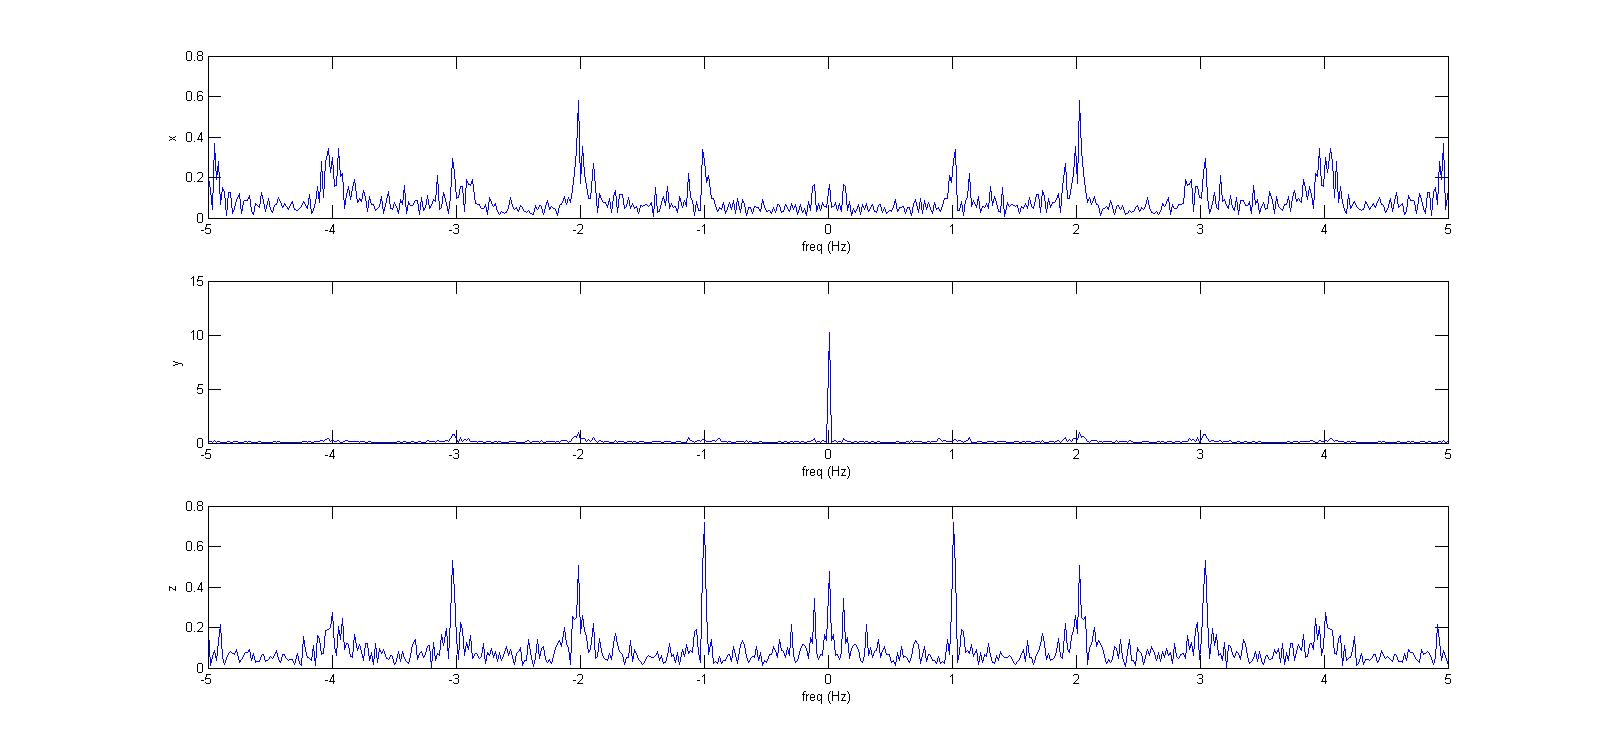
\includegraphics[width=3.5in]{figures/AccFreq}
	\caption{Accelerometer readings in frequency domain}
\end{figure}

We try to calculate our speed using the accelerometer readings. 
This is feasible theoretically if the speed is always zero at the starting point. 
But in practical, we met way more challenges while trying to implement this method.

The first challenge was the accuracy of sensor readings.
Since 0.1m/s\^2 errors at acceleration will accumulate to 1m/s error at velocity during 10 seconds, if we consider the error is constant, this will lead to a 5m error at the location.
Although we have tested that the sensor readings are quite stable while the smartphone is static. 
Since trivial errors in accelerometer readings will lead to very significant location errors, we have to reconsider this problem.
In our sensor reading accuracy tests, we put it on the desk to see the changes of the sensor readings. 
The errors of sensor readings keep changing, sometimes it can reach up to 0.3m/s\^s. 
These errors will finally lead up to tens or even hundreds of meters error in localization results during a short measure only lasting for tens of seconds.

The second challenge we met is that to calculate the speed using the accelerometer readings, we need to deal with the gravity, which dominate the sensor readings.
Since all we want is the speed moving forward, but we can hardly known the relative direction of the gravity in advance. 
This means it's difficult to get rid of it from sensor readings.
Also, in practice, when people carrying the phone are moving, they are more likely to put them in their pocket.
In this case, the direction of gravity contrast to smartphone orientation are changing dynamically, it is almost impossible for us to calculate its relative direction.

The last challenge we found is that there is too much noise introduced by shocks of smartphones. 
As we discussed before, people tend to put their phone in their pockets, and the smartphone will shock in their pockets.
We have used FFT to analyze the sensor readings at frequency domain. 
The signal in the frequency domain show in Fig.12 yield that, without any luck, these noises are everywhere and difficult to remove.
Considering that the forward acceleration of a person moving forward is so less significant compared to the noise generated by all kinds of shocks of smartphones, as far as we know, we don't see any signal processing technologies that can possibly obtain the signal (forward acceleration) among big noises (different kinds of shocks of smartphones).

In conclusion, calculating the forward speed from sensor readings is really difficult, as far as we know, there is no signal processing technology that can do this.
Considering the moving patterns of different kinds of people movements (a lot of shocks and little forward acceleration for walking, medium shocks and larger acceleration for biking, small shocks and large acceleration for skiing), we deal with different kinds of sports separately.
We deal with the most common cases, walking, in our system first.
Since biking has a similar pattern as walking, we are thinking of using similar methods to deal with them both.

Since it's so difficult for us to calculate the forward acceleration through the accelerometer readings, we will use a different method for walking.
By doing several experiments, we found that the accumulated forward acceleration of a walking person is almost zero.
Considering that we are walking at constant speed for most of the time, always treating the forward acceleration as zero seems feasible.
There are some studies about speed and step in the literature.
From their result, we can see that under certain speed, the relation of speed and step frequency is almost linear \cite{Speed and Step}.
So we calculate the forward speed of a walking person by identifying and counting his steps.
In a regular situation, the step size of a person is almost stable.
It varies in some cases such as when going up a hill, but on a flat ground, it is likely stable.
Although we can use the similar method for recording biking paths, the result may not be precise due to the step size of biking is not as stable as walking, since the speed of biking is not constant.
Also the step size of biking is difficult to train, so this requires some more complicated mechanisms.
Currently we haven't implemented this part in our system.

For the step size, we can use some predefined values calculated from some parameters such as the height, gender and age of a person. 
There are some recommended values and tables out there.
A better approach is that we can always use the GPS to help to calibrate these predefined values.
This will make the system more adaptive since people tend to change their step size in different conditions (i.e. raining or snowing days, outdoor or indoor scenarios, ascending or descending trails)

From analysis of the sensor readings while we are walking, we see that the axis which near the direction of gravity most, has the largest variance during walking.
Large variances mean it is easier to identify steps with few possible false positives.
So the axis near the direction of gravity most is the most suitable one for us to identifying steps from sensor readings.

To deal with false positives of step counting, we introduce two mechanisms in our system.
The first one is that we borrow the idea of hysteresis comparator.
We calculate the mean value on the axis we choose to use first.
Then we use some predefined threshold to identify the steps.
Such as when the readings are higher than the mean value plus the threshold, we treat it as the person is lifting their one foot.
When the readings are lower than the mean value subtract the threshold, we treat it as the person is putting down their foot.
We can use sqrt(2)/2 as the predefined threshold, note that with a higher threshold, we certainly can reduce most false positives, but at the mean time, we will fail to count some steps.
Note that even high quality commercial step counter are suffering from some false positives, it is impossible to totally avoid this issue when using accelerometers.\cite{Motion Sensor Accuracy}.
Reference \cite{Gyroscope Step Count} has proposed to count the step using gyroscope.
Actually this is a more precise way to count step, but the algorithm in that paper is kind of complex, and the method is similar with using accelerometers, so we stick to accelerometers in our test.
We can always calibrate the threshold when the system is running.
The second one is that a person's step frequency is in a certain range.
It will neither be too high nor too low.
With this knowledge, we can set up a shock resistance system that filter out some high frequency shocks and low frequency shocks.
In our specific design, it works as follows: when the step state is changing to "lifting a foot" the state will not change to "putting down a foot" until a certain delay has been reached.

\subsubsection{Interpreting the magnetometer data}
\begin{figure}
	\centering
	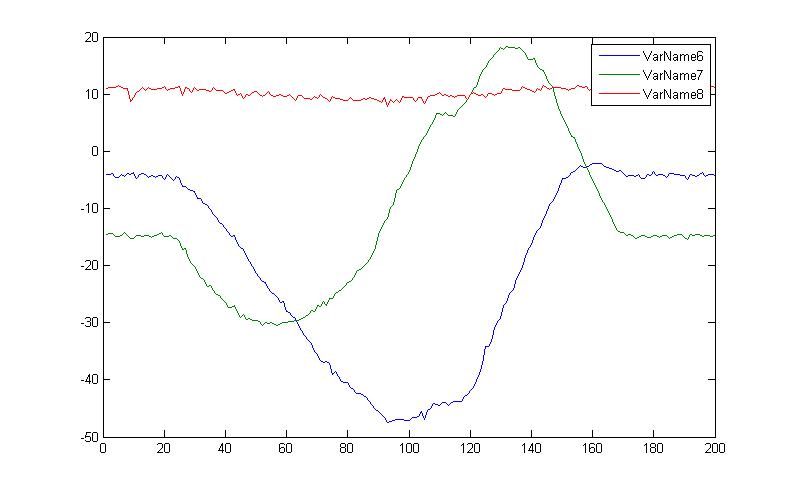
\includegraphics[width=3.5in]{figures/mag-flat}
	\caption{Magnetometer readings when we change the orientation of a smartphone in a 2-D circle}
	\includegraphics[width=3.5in]{figures/indoor-flat-mag}
	\caption{Magnetometer readings when we hold a smartphone and walk in Min Kao where there is metal guard bars}
\end{figure}

We uses magnetometer readings to calculate our directions and changes of it.
Fig.13 shows the change of the magnetometer readings when the phone is flat on a desk and its orientation has been changed continuously for a whole circle.
Note that we start moving it around sample 20 and stop moving it around sample 165.
One axis is almost not changed because we are moving the orientation of the smartphone only in 2-D.
We use a totally different method to deal with noises for magnetometer readings interpreting.
The first is that we use the mean values of readings of a single step to calculate the direction of this step.
Although the magnetometer readings also have a lot of noise introduced by shocks, considering that if we are going straight, the magnetometer readings should not be changing at all, which means all the noises are periodical and their periods are a single step.
So simply using integration (get the mean value), we can remove most of the errors introduced by noises.
But even when we are using average values, it seems that the errors of magnetometer readings on smartphones are more significant than errors of accelerometers, so we have to use some approximations to deal with this.
Since the readings are changing even when we are not moving our smartphone, we collect the reading errors when the smartphone is placed flat, and we can only map the readings to limited discrete directions because of these errors.
The case is even worse when the smartphone is moving.
Actually even a compass is changing constantly when you are walking with it.
You can not read the direction unless you stop and wait for it to be stable.
So to deal with this character of magnetometer readings, we will only map them into four or eight directions, and we can always use the GPS to calibrate our actual direction of movement.

Another challenge is that the magnetic field is affected by obstacles such as metal, walls. 
This characteristic makes it so much harder to calculate the direction for indoor scenarios.
Fig.14 shows the magnetometer readings when we hold the phone to waking a rectangle in fourth floor of Min Kao where there are metal guard bars. 
Compared to Fig.7 which also reflect a test in Min Kao which is not in an area near metal guard bars, we can see that the result are inconsistent.
We may draw some useful information from Fig.7 but it is almost impossible to draw any useful information from Fig.14.
Currently, we haven't found a good approach to deal with this, so our system can only work in outdoor scenarios.
Microsoft research asia has also developed a similar algorithm as ours, but they use it for indoor localization \cite{MSRA Similar Work}.
From their analysis, the orientation detection using magnetometer is still an open issue in their system.
Even for outdoor scenarios, the magnetometer readings vary at different places, which requires calibration before using it.
Based on our observation of a large number of experiments, we found that the magnetic field is pretty stable at any given outdoor scenario.
Although they might be changing a little bit during different times of a day, they are quite stable for a pretty long period.

We can conclude from our observations that a calibration is always needed.
If we are not moving too far, we only need to calibrate at the very beginning.
But when the trip is really long, we may need to calibrate the magnetometer readings on the run.
The good news is that the calibration of magnetometer is pretty simple. 
We do not even need to spend any time for calibration on the run, this can be done by simply using the history records.
There are two parameters we need to calibrate, one is the magnetometer readings range, another is the magnetometer readings shift.
The former one is the magnetometer reading's range when you change the orientation of your phone around a certain axis.
The latter one is the lowest magnetometer readings when you change the orientation of your phone around a certain axis.
So all we need to do to calibrate our magnetometer readings is to move our smartphone around a circle.
This is why if we want to calibrate the readings on the run, we can simply collect these two parameters during our walk.
\subsubsection{Mapping the sensor readings into the change of coordinates}
Our system using the GPS to get the initial coordinates.
After that, we calculate the moving speed and moving direction from the sensor readings, and map these changes into coordinate changes.
For example, if we change only map the magnetometer readings into four directions, for each step, we can change the coordinates in the following way:
\begin{itemize}
	\item west: 

		minus the longitude by the step size
	\item north: 

		plus the latitude with the step size
	\item south: 

		minus the latitude by the step size
	\item east: 

		plus the longitude with the step size
\end{itemize}

If we map the magnetometer readings in to eight or more directions, we can always using such a method to approximate the coordinates changes.

We notice that if we are going on a direction such that the magnetometer readings are on the boundary of two adjacent directions, the direction may change frequently due to the randomness of magnetometer readings.
So we can add some protection areas between adjacent directions. 
When the magnetometer readings fall into these categories, there are two mechanisms we can adopt.
The first one is that we simply don't count current step.
This method will lose some steps, but it will generate a path on the map with a similar shape compared to the correct one.
The other method is to using the former direction, which means that if the change of the magnetometer readings are not changing significantly enough, we simply not change direction.
This is a similar idea as we borrow from the hysteresis comparator to deal with accelerometer readings.
\subsection{Map integrator}
There are some Android development APIs can simply using the coordinates we generate to draw dots on the map and connect them with lines \cite{Google Map APIs}.
This procedure can also works in an online way, which uses some animations to show current locations and previous path.
Unfortunately, since this project is an idea proven project, and we are using Python instead of Java, which lacking such map APIs, we are unable to do that in our system.
We use Javascript to write a separate program to read the coordinates our system generated and draw them on a map. 
Currently, our map integrator can only work in an offline mode which requires all the coordinates generated by the system and draw them on a map.
Since all our coordinates are generated in an online approach as well as the output file (whenever a new coordinates has been generated, the system will append the output file with a new coordinates), it requires very little effort for one with enough knowledge of Android development with Java to implement and online map integrator.
Why do we still want to use Python instead of Java? We will explain that later.
\subsection{GPS coordinator}
\begin{figure}
	\centering
	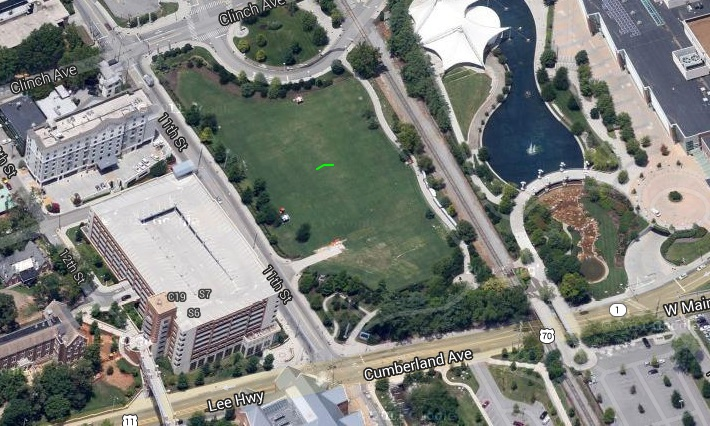
\includegraphics[width=3.5in]{figures/gps-test-stand}
	\caption{GPS results when stand still for one minute}
	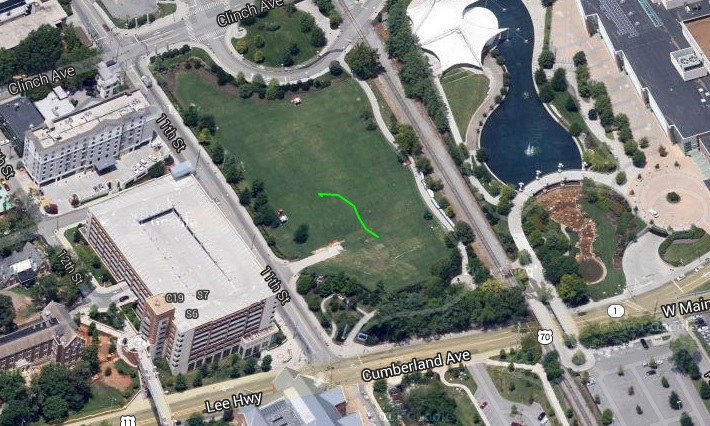
\includegraphics[width=3.5in]{figures/gps-test}
	\caption{GPS results when walk in a straight line for one minute}
\end{figure}

Sensors can only be used to describe our movements.
To determine our location, we need at least an initial location.
We use the GPS to get the initial location, while for some scenarios when the GPS signal is very weak or not available at all, we can also use some alternative sources such as the network to get the initial location.

We use the GPS to calibrate the coordinates when magnetometer readings are changing significantly.
But sometimes GPS requires quite a long time to return the new coordinates which makes it impractical for short tracks.
GPS return value may not reflect the current value, but there is a time stamp provided along with the coordinates. 
We can use this time stamp to calculate the error of coordinates at specific times and then offset the current value to make up the error. 
Since in our approach, errors are accumulated linearly.

Since GPS results really need a long time to achieve a high level of accuracy, it is not practical to use it for calibration for short tracks.
Fig.15 shows the GPS results when we stand still in one minute. 
Fig.16 shows the GPS results when we walk in a straight line in one minute.
Results of both figure imply that the GPS results need a quite long time to achieve a high level of accuracy.

\subsection{Central controller}
The original design of central controller should connect all three parts together.
Since Python on Android lack some of the required map APIs, so currently only our central controller only contains sensor data interpreter and GPS coordinator.
The central controller can run as a background service and will append current coordinates to a file, which can be read dynamically by other programs to show the path in real-time.
\subsection{Why do we still want Python?}
Google employees have developed an App called script layer for Android (SL4A) \cite{SL4A}, and Python for Android is one supported programming language of SL4A.
SL4A also makes it possible to use several different kinds of scripting languages for Android development.
Python for Android provided a wide range of APIs for developers to do almost everything Java can do on a smartphone.
But they are still lacking some APIs, such as map related APIs which we want to use in our system.
In spite of this disadvantage, there are still a lot of great advantages that makes us want to use Python in developing our system.
To name a few:
\begin{itemize}
	\item Easy to debug in real environment: 

		Consider this situation, we want to choose the value of a specific parameter in our system.
		For Java development:
		We set an initial one, and go to where we want to test (such as a lawn outside), we found the value needed to be changed.
		What should we do?
		We need go back to our office, change the source code, compile it and download to our smartphone.
		We need to iterate this step if we want to make further modification.
		For Python development:
		All we need is to open the script with any plain text editor on your phone and run it immediately!
	\item Short code size: 
		
		For the same functionality, the Python code is only one fifth as long as the Java code \cite{PvJ}.
		The code size of all our test is only 141 lines!
	\item A language that match your mental representation most: 
		
		Isn't that great? Read this article online \cite{Why Python}, start to use Python today!
\end{itemize}
\section{Evaluation}
We have implemented our system and test them in real environments. 
We designed four tests, we walked in some certain pattern so that the path will show some "fancy" patterns on the map. 
We evaluate the performance (correctness of the result, precision) of sensors in this way.

Since the energy consumption is a concern to many parts of a running system as well as different smartphones and its operating system. 
It's really difficult for us to quantify our energy savings.
But since our system use GPS for very limited time, and from our early discussion that compared to GPS, sensors only consumes negligiblg energy, so the energy efficiency is higher when only considering the GPS usage.

Comparing Fig.17, Fig.18, Fig.19 and Fig.20 with Fig.15 and Fig.16, we can see that sensors are more responsive than GPS. 
All the test with sensors are less than 1 minute, we can make a lot of turns and the sensors can show them with an acceptable level of accuracy.
But GPS takes one minute and only generates 4-5 results.
This makes the sensors more suitable for some real-time applications, such as aerial photography.
\subsection{Compromises of the experiments}
Since this is an idea proven system, we have several compromises to make our system simple yet still can prove our idea.
We made following compromises:
\begin{itemize}
	\item hold the smartphone in the hand: 

		This can simplify our step counter program since the accelerometer readings have much less noise. 
		In this case, we reduce the effort to deal with false positives introduced by shocks of smartphones when it is in our pockets.
	\item only for outdoor scenario: 

		Our system currently can only work in outdoor scenarios, where the magnetic field density is rather constant. 
		Indoor scenarios often raise the requirement to deal with the non-constant magnetic field.
	\item short tracks: 

		We only test our system in short tracks.
		In this case, we only need to calibrate the magnetometer readings at the beginning of the test.
		We haven't implemented on the run calibration in our current system.
	\item no GPS calibration: 

		We only use the GPS to acquire coordinates of the initial location.
		Since our tests only include short tracks, and GPS calibration requires a pretty long time thus is only worthwhile for long tracks, so we don't use the GPS to calibrate our result during the test.
		The disadvantage of this compromise is that when there is a large error on our initial location acquired from the GPS, there is no way for us to correct it during the test.

	\item adjust the system parameters for each person:

		We haven't written the code to get system parameters (which vary from different person) during the test.
		Instead, we use predefined values for each person.
		For example, we use predefined step size recommended by some commercial step counter. 
		And we don't use the GPS to calibrate this parameter during the test.
\end{itemize}

\subsection{Extras}
There are some other less significant issues during our test:
\begin{itemize}
	\item the wake lock: 

		There is no sensor readings after the screen is turned off.
		It seems the sensor reading providers are stop working during that time.
		So we use wake lock to keep the system from sleep.
	\item effect of different kinds of smartphone cases: 

		During our test, we found that the material of smartphone cases may affect the performance of magnetometer readings.
		Smartphones with metal cases (such as Lenovo K900 \cite{K900}) has worse magnetometer performance than smartphones with plastic cases (such as Nexus 4 \cite{Nexus 4}).
\end{itemize}

\subsection{Three experiments and a trekking}
We have three walking tests and a biking test.

\subsubsection{Rectangle}
\begin{figure}
	\centering
	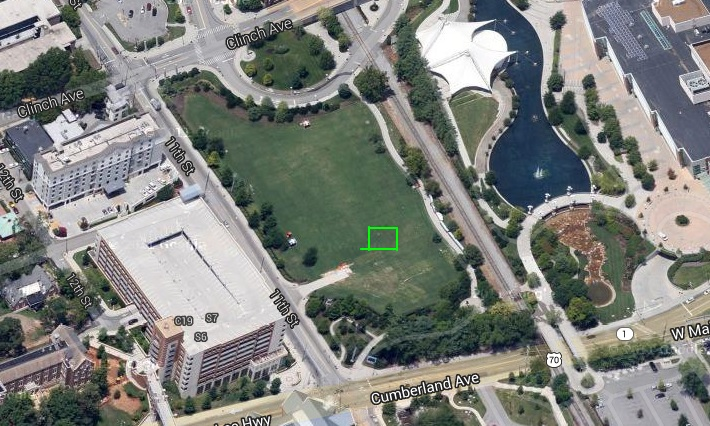
\includegraphics[width=3.5in]{figures/1-rect}
	\caption{Test result for walking as a rectangle}
\end{figure}

The tester holds the smartphone and walks as a rectangle pattern.
The result is shown in Fig.17.
We can see that the sensor readings can achieve a pretty high level of accuracy when the system parameters have been well tuned.

\subsubsection{"Gong"}
\begin{figure}
	\centering
	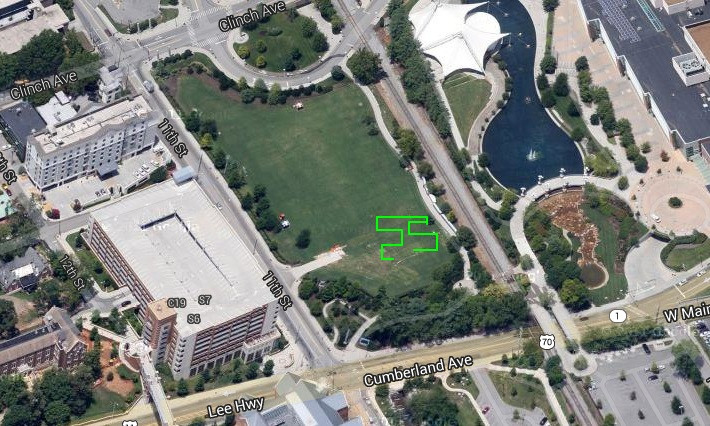
\includegraphics[width=3.5in]{figures/2-gong}
	\caption{Test result for walking as a Chinese character "Gong"}
\end{figure}

The tester holds the smartphone and walks as a Chinese character "Gong" pattern.
The result is shown in Fig.18.
There is a quite large error in coordinates of initial location, but we can not correct it only using sensor readings.
In this case, all the recorded path has been shifted with the same offset, which is the initial error of GPS results.

\subsubsection{Spiral}
\begin{figure}
	\centering
	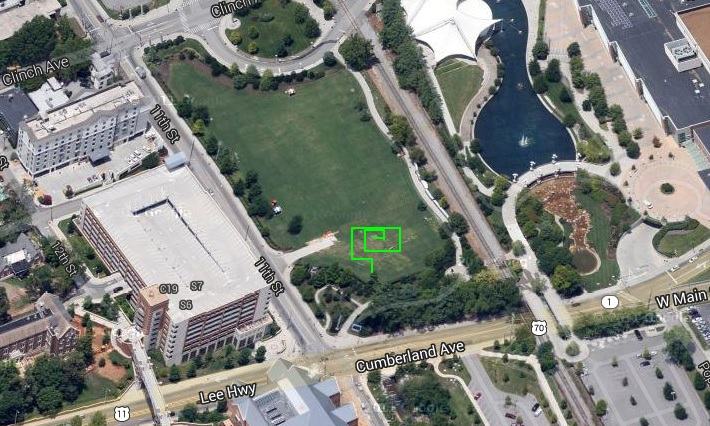
\includegraphics[width=3.5in]{figures/3-circle}
	\caption{Test results for walking as a spiral pattern}
\end{figure}

The tester holds the smartphone and walks as a spiral pattern.
The result is shown in Fig.19.
Since we are discarding steps which orientation falls in protection area, so we can see some missing steps in this test result.
The tester is trying to walk a larger outside rectangle, but we can see from Fig.19 that the north edge of the two rectangles are almost overlapped.

\subsubsection{Trekking}
\begin{figure}
	\centering
	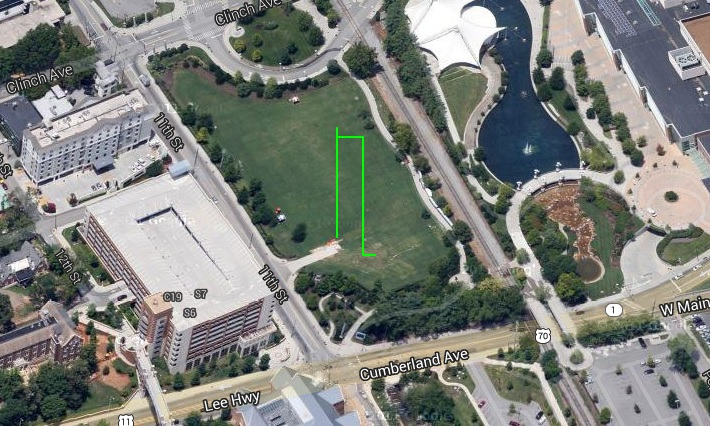
\includegraphics[width=3.5in]{figures/4-biking}
	\caption{Test results for ridding a bike}
\end{figure}

The tester holds the smartphone and riding a bike following a simple pattern, the step size and step count threshold is tuned to biking scenario.
The result is shown in Fig.20.
Note that the upper left corner has a small jitter, that imply a wrong orientation detection.
It should make clear that the lower right corner also has a small jitter, but it is caused by the rider's is not holding the smartphone horizontally when he got on the bike.

\section{Conclusion}
Motion sensors are widely available on smartphones recently.
We propose to use sensor readings to describe our movements to assist in localization.
We implemented a test application for path recording using sensors and the GPS cooperatively.
Our test system is specialized for walking scenarios which can also apply to simple biking scenarios with minor changes.
Our results show that sensors can achieve a quite high level of accuracy and with a large advantage in terms of energy efficiency and latency.
Nevertheless, sensors themselves can only describe movements, without GPS results they can not map movements into coordinates changes.

\section*{Acknowledgment}
The authors would like to thank Dr. Gao for illuminating advises he gave during our groping of cool ideas.

% Can use something like this to put references on a page
% by themselves when using endfloat and the captionsoff option.
\ifCLASSOPTIONcaptionsoff
  \newpage
\fi

\begin{thebibliography}{1}

\bibitem{GPS}
	https://en.wikipedia.org/wiki/GPS
\bibitem{A-GPS}
	https://en.wikipedia.org/wiki/Assisted\_GPS
\bibitem{Sensor Aug}
	Ofstad, Andrew, et al. "Aampl: Accelerometer augmented mobile phone localization." Proceedings of the first ACM international workshop on Mobile entity localization and tracking in GPS-less environments. ACM, 2008.
\bibitem{Track for Mobile}
	Thiagarajan, Arvind, et al. "Accurate, low-energy trajectory mapping for mobile devices." Proceedings of the 8th USENIX conference on Networked systems design and implementation. USENIX Association, 2011.
\bibitem{GPS Latency}
	Eric S. Raymond. "Performance analysis of GPSes and GPSD." http://www.catb.org/gpsd/performance.html
\bibitem{GPS Measurements}
	Lin, Kaisen, et al. "Energy-accuracy aware localization for mobile devices." Proceedings of 8th International Conference on Mobile Systems, Applications, and Services (MobiSys’ 10). 2010.
\bibitem{Acc Measurements}
	STMicroelectronics. "LIS331DLH MEMS digital output motion sensor ultra low-power high performance 3-axiss "nano" accelerometer datasheet." July, 2009.
\bibitem{Speed and Step}
	Rowlands, Ann V., Michelle R. Stone, and Roger G. Eston. "Influence of speed and step frequency during walking and running on motion sensor output." Medicine and science in sports and exercise 39.4 (2007): 716.
\bibitem{Motion Sensor Accuracy}
	Le Masurier, Guy C., SARAH M. Lee, and C. A. T. R. I. N. E. Tudor-Locke. "Motion sensor accuracy under controlled and free-living conditions." Medicine and Science in Sports and Exercise 36.5 (2004): 905-910.
\bibitem{Gyroscope Step Count}
	Pappas, Ion PI, et al. "A reliable gyroscope-based gait-phase detection sensor embedded in a shoe insole." Sensors Journal, IEEE 4.2 (2004): 268-274.
\bibitem{MSRA Similar Work}
	Li, Fan, et al. "A reliable and accurate indoor localization method using phone inertial sensors." Proceedings of the 2012 ACM Conference on Ubiquitous Computing. ACM, 2012.
\bibitem{Google Map APIs}
	Google. "Google Map API documentation for JavaScript: https://developers.google.com/maps/documentation/javascript/" 
\bibitem{SL4A}
	Ferrill, Paul. "Pro Android Python with SL4A." Apress, 2011.
\bibitem{PvJ}
	Leif Johnson. "Python vs. Java", Mar 2003.
\bibitem{Why Python}
	Eric S. Raymond. "Why Python?" LINUX Journal issue \#73, May 2000
\bibitem{K900}
	Lenovo. "Lenovo K900 datasheet.", Lenovo, 2012
\bibitem{Nexus 4}
	LG. "LG E960 Nexus 4 datasheet.", LG, 2012


\end{thebibliography}


% that's all folks
\end{document}


